Sei
\[
{ALL}_{\text{DEA}}=\{\, \langle A\rangle\, |\, \text{$A$ ist ein DEA und $L(A)=\Sigma^*$}\}.
\]
Zeigen sie:
$ALL_{\text{DEA}}$ ist entscheidbar.

\thema{Entscheidbarkeit}

\begin{loesung}
Drei mögliche Lösungen:
\begin{enumerate}
\item
Der folgende Algorithmus entscheidet: Bilde den minimalen Automaten von
$A$ und akzeptiere, falls $A$ der Automat
\begin{center}
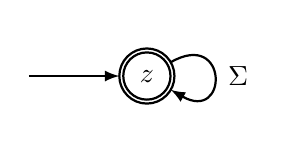
\begin{tikzpicture}[>=latex,thick]
\draw[->,shorten >= 0.35cm] (-1.5,0) -- (0,0);
\draw (0,0) circle[radius=0.35];
\draw (0,0) circle[radius=0.30];
\node at (0,0) {$z\mathstrut$};
\draw[->,shorten >= 0.35cm,shorten <= 0.35cm]
	(0,0) to[out=30,in=-30,distance=1.2cm] (0,0);
\node at (0.9,0) [right] {$\Sigma$};
\end{tikzpicture}
\end{center}
%\[
%\entrymodifiers={++[o][F]}
%\xymatrix{
%*+\txt{}\ar[r]
%        &*++[o][F=]{z}\ar@(ur,dr)^{*}
%}
%\]
ist.
\item
Der folgende Algorithmus entscheidet: bilde den Automaten, der
$\overline{L(A)}$ akzeptiert (dieser Automat existiert, weil
das Komplement einer regulären Sprache wieder regulär ist)
und wende den Entscheider von $E_\text{DEA}$ darauf an.
\item
$\Sigma^*$ ist regulär, es gibt also einen Automaten $B$, der
$\Sigma^*$ akzeptiert. Jetzt wendet man den Entscheider von
$\text{\it EQ}_{\text{DEA}}$ auf $A$ und $B$ an, und akzeptiert,
wenn dieser akzeptiert. Andernfalls verwirft man.
\qedhere
\end{enumerate}
\end{loesung}
